% Graphic for TeX using PGF
% Title: C:\Users\Ahmet\Desktop\BachelorArbeit\ausarbeitung_tex_kit_2016\Ausarbeitung_TeX_KIT\designs\perceptron_2ein_2aus.dia
% Creator: Dia v0.97.2
% CreationDate: Wed Feb 12 21:12:48 2020
% For: Ahmet
% \usepackage{tikz}
% The following commands are not supported in PSTricks at present
% We define them conditionally, so when they are implemented,
% this pgf file will use them.
\ifx\du\undefined
  \newlength{\du}
\fi
\setlength{\du}{15\unitlength}
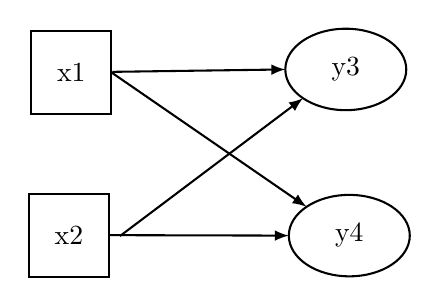
\begin{tikzpicture}
\pgftransformxscale{1.000000}
\pgftransformyscale{-1.000000}
\definecolor{dialinecolor}{rgb}{0.000000, 0.000000, 0.000000}
\pgfsetstrokecolor{dialinecolor}
\definecolor{dialinecolor}{rgb}{1.000000, 1.000000, 1.000000}
\pgfsetfillcolor{dialinecolor}
\pgfsetlinewidth{0.050000\du}
\pgfsetdash{}{0pt}
\pgfsetdash{}{0pt}
\pgfsetbuttcap
\pgfsetmiterjoin
\pgfsetlinewidth{0.050000\du}
\pgfsetbuttcap
\pgfsetmiterjoin
\pgfsetdash{}{0pt}
\definecolor{dialinecolor}{rgb}{1.000000, 1.000000, 1.000000}
\pgfsetfillcolor{dialinecolor}
\fill (5.032260\du,6.100000\du)--(5.032260\du,8.100000\du)--(6.967744\du,8.100000\du)--(6.967744\du,6.100000\du)--cycle;
\definecolor{dialinecolor}{rgb}{0.000000, 0.000000, 0.000000}
\pgfsetstrokecolor{dialinecolor}
\draw (5.032260\du,6.100000\du)--(5.032260\du,8.100000\du)--(6.967744\du,8.100000\du)--(6.967744\du,6.100000\du)--cycle;
\pgfsetbuttcap
\pgfsetmiterjoin
\pgfsetdash{}{0pt}
\definecolor{dialinecolor}{rgb}{0.000000, 0.000000, 0.000000}
\pgfsetstrokecolor{dialinecolor}
\draw (5.032260\du,6.100000\du)--(5.032260\du,8.100000\du)--(6.967744\du,8.100000\du)--(6.967744\du,6.100000\du)--cycle;
\pgfsetlinewidth{0.050000\du}
\pgfsetdash{}{0pt}
\pgfsetdash{}{0pt}
\pgfsetbuttcap
\pgfsetmiterjoin
\pgfsetlinewidth{0.050000\du}
\pgfsetbuttcap
\pgfsetmiterjoin
\pgfsetdash{}{0pt}
\definecolor{dialinecolor}{rgb}{1.000000, 1.000000, 1.000000}
\pgfsetfillcolor{dialinecolor}
\fill (4.975000\du,10.020000\du)--(4.975000\du,12.020000\du)--(6.910484\du,12.020000\du)--(6.910484\du,10.020000\du)--cycle;
\definecolor{dialinecolor}{rgb}{0.000000, 0.000000, 0.000000}
\pgfsetstrokecolor{dialinecolor}
\draw (4.975000\du,10.020000\du)--(4.975000\du,12.020000\du)--(6.910484\du,12.020000\du)--(6.910484\du,10.020000\du)--cycle;
\pgfsetbuttcap
\pgfsetmiterjoin
\pgfsetdash{}{0pt}
\definecolor{dialinecolor}{rgb}{0.000000, 0.000000, 0.000000}
\pgfsetstrokecolor{dialinecolor}
\draw (4.975000\du,10.020000\du)--(4.975000\du,12.020000\du)--(6.910484\du,12.020000\du)--(6.910484\du,10.020000\du)--cycle;
% setfont left to latex
\definecolor{dialinecolor}{rgb}{0.000000, 0.000000, 0.000000}
\pgfsetstrokecolor{dialinecolor}
\node at (6.000000\du,7.100000\du){x1};
% setfont left to latex
\definecolor{dialinecolor}{rgb}{0.000000, 0.000000, 0.000000}
\pgfsetstrokecolor{dialinecolor}
\node at (5.942740\du,11.020000\du){x2};
\definecolor{dialinecolor}{rgb}{1.000000, 1.000000, 1.000000}
\pgfsetfillcolor{dialinecolor}
\pgfpathellipse{\pgfpoint{12.613479\du}{7.028296\du}}{\pgfpoint{1.456779\du}{0\du}}{\pgfpoint{0\du}{0.981096\du}}
\pgfusepath{fill}
\pgfsetlinewidth{0.050000\du}
\pgfsetdash{}{0pt}
\pgfsetdash{}{0pt}
\definecolor{dialinecolor}{rgb}{0.000000, 0.000000, 0.000000}
\pgfsetstrokecolor{dialinecolor}
\pgfpathellipse{\pgfpoint{12.613479\du}{7.028296\du}}{\pgfpoint{1.456779\du}{0\du}}{\pgfpoint{0\du}{0.981096\du}}
\pgfusepath{stroke}
\definecolor{dialinecolor}{rgb}{1.000000, 1.000000, 1.000000}
\pgfsetfillcolor{dialinecolor}
\pgfpathellipse{\pgfpoint{12.697979\du}{11.031196\du}}{\pgfpoint{1.456779\du}{0\du}}{\pgfpoint{0\du}{0.981096\du}}
\pgfusepath{fill}
\pgfsetlinewidth{0.050000\du}
\pgfsetdash{}{0pt}
\pgfsetdash{}{0pt}
\definecolor{dialinecolor}{rgb}{0.000000, 0.000000, 0.000000}
\pgfsetstrokecolor{dialinecolor}
\pgfpathellipse{\pgfpoint{12.697979\du}{11.031196\du}}{\pgfpoint{1.456779\du}{0\du}}{\pgfpoint{0\du}{0.981096\du}}
\pgfusepath{stroke}
\pgfsetlinewidth{0.050000\du}
\pgfsetdash{}{0pt}
\pgfsetdash{}{0pt}
\pgfsetbuttcap
{
\definecolor{dialinecolor}{rgb}{0.000000, 0.000000, 0.000000}
\pgfsetfillcolor{dialinecolor}
% was here!!!
\pgfsetarrowsend{latex}
\definecolor{dialinecolor}{rgb}{0.000000, 0.000000, 0.000000}
\pgfsetstrokecolor{dialinecolor}
\draw (6.992691\du,7.086197\du)--(11.156700\du,7.028300\du);
}
\pgfsetlinewidth{0.050000\du}
\pgfsetdash{}{0pt}
\pgfsetdash{}{0pt}
\pgfsetbuttcap
{
\definecolor{dialinecolor}{rgb}{0.000000, 0.000000, 0.000000}
\pgfsetfillcolor{dialinecolor}
% was here!!!
\pgfsetarrowsend{latex}
\definecolor{dialinecolor}{rgb}{0.000000, 0.000000, 0.000000}
\pgfsetstrokecolor{dialinecolor}
\draw (6.910480\du,11.020000\du)--(11.241200\du,11.031200\du);
}
\pgfsetlinewidth{0.050000\du}
\pgfsetdash{}{0pt}
\pgfsetdash{}{0pt}
\pgfsetbuttcap
{
\definecolor{dialinecolor}{rgb}{0.000000, 0.000000, 0.000000}
\pgfsetfillcolor{dialinecolor}
% was here!!!
\pgfsetarrowsend{latex}
\definecolor{dialinecolor}{rgb}{0.000000, 0.000000, 0.000000}
\pgfsetstrokecolor{dialinecolor}
\draw (6.967740\du,7.100000\du)--(11.667900\du,10.337500\du);
}
\pgfsetlinewidth{0.050000\du}
\pgfsetdash{}{0pt}
\pgfsetdash{}{0pt}
\pgfsetbuttcap
{
\definecolor{dialinecolor}{rgb}{0.000000, 0.000000, 0.000000}
\pgfsetfillcolor{dialinecolor}
% was here!!!
\pgfsetarrowsend{latex}
\definecolor{dialinecolor}{rgb}{0.000000, 0.000000, 0.000000}
\pgfsetstrokecolor{dialinecolor}
\draw (7.172880\du,11.041900\du)--(11.583400\du,7.722040\du);
}
% setfont left to latex
\definecolor{dialinecolor}{rgb}{0.000000, 0.000000, 0.000000}
\pgfsetstrokecolor{dialinecolor}
\node at (12.613500\du,7.028300\du){y3};
% setfont left to latex
\definecolor{dialinecolor}{rgb}{0.000000, 0.000000, 0.000000}
\pgfsetstrokecolor{dialinecolor}
\node at (12.698000\du,11.031200\du){y4};
\end{tikzpicture}
